\subsection{Use Cases}
For at sikre at vi laver et program, der fungerer som ønsket, har vi opstillet flere use cases for systemet.
Disse use cases er blevet udledt på baggrund af møder med Psykolog Nords ledelse, og ved brug af de fire basis funktioner for persistens: create, read, update og delete (CRUD), på objekt- og domænemodelen.
Derudover har vi også identificeret primæraktørene og deres mål, og sikret at vores use cases opfylder målene.

Vores primæraktører og deres mål er:

\begin{itemize}
    \item Booker
        \begin{itemize}
            \item Se aftaler
            \item Book aftale
            \item Ændr aftale
            \item Aflys aftale
        \end{itemize}
    \item Behandler
        \begin{itemize}
            \item Læs klients journal
            \item Ajourfør klients journal
        \end{itemize}
    \item Klient
        \begin{itemize}
            \item Se og betal fakturaer
        \end{itemize}
    \item Superbruger
        \begin{itemize}
            \item Håndter bruger
            \item Håndter brugers rettigheder
        \end{itemize}

\end{itemize}

Det er f.eks. vigtigt at skelne mellem at booke en ny aftale, ændre den og aflyse den, da det er tre forskellige funktionaliteter i systemet.

\begin{figure}[p]
	\centering
  		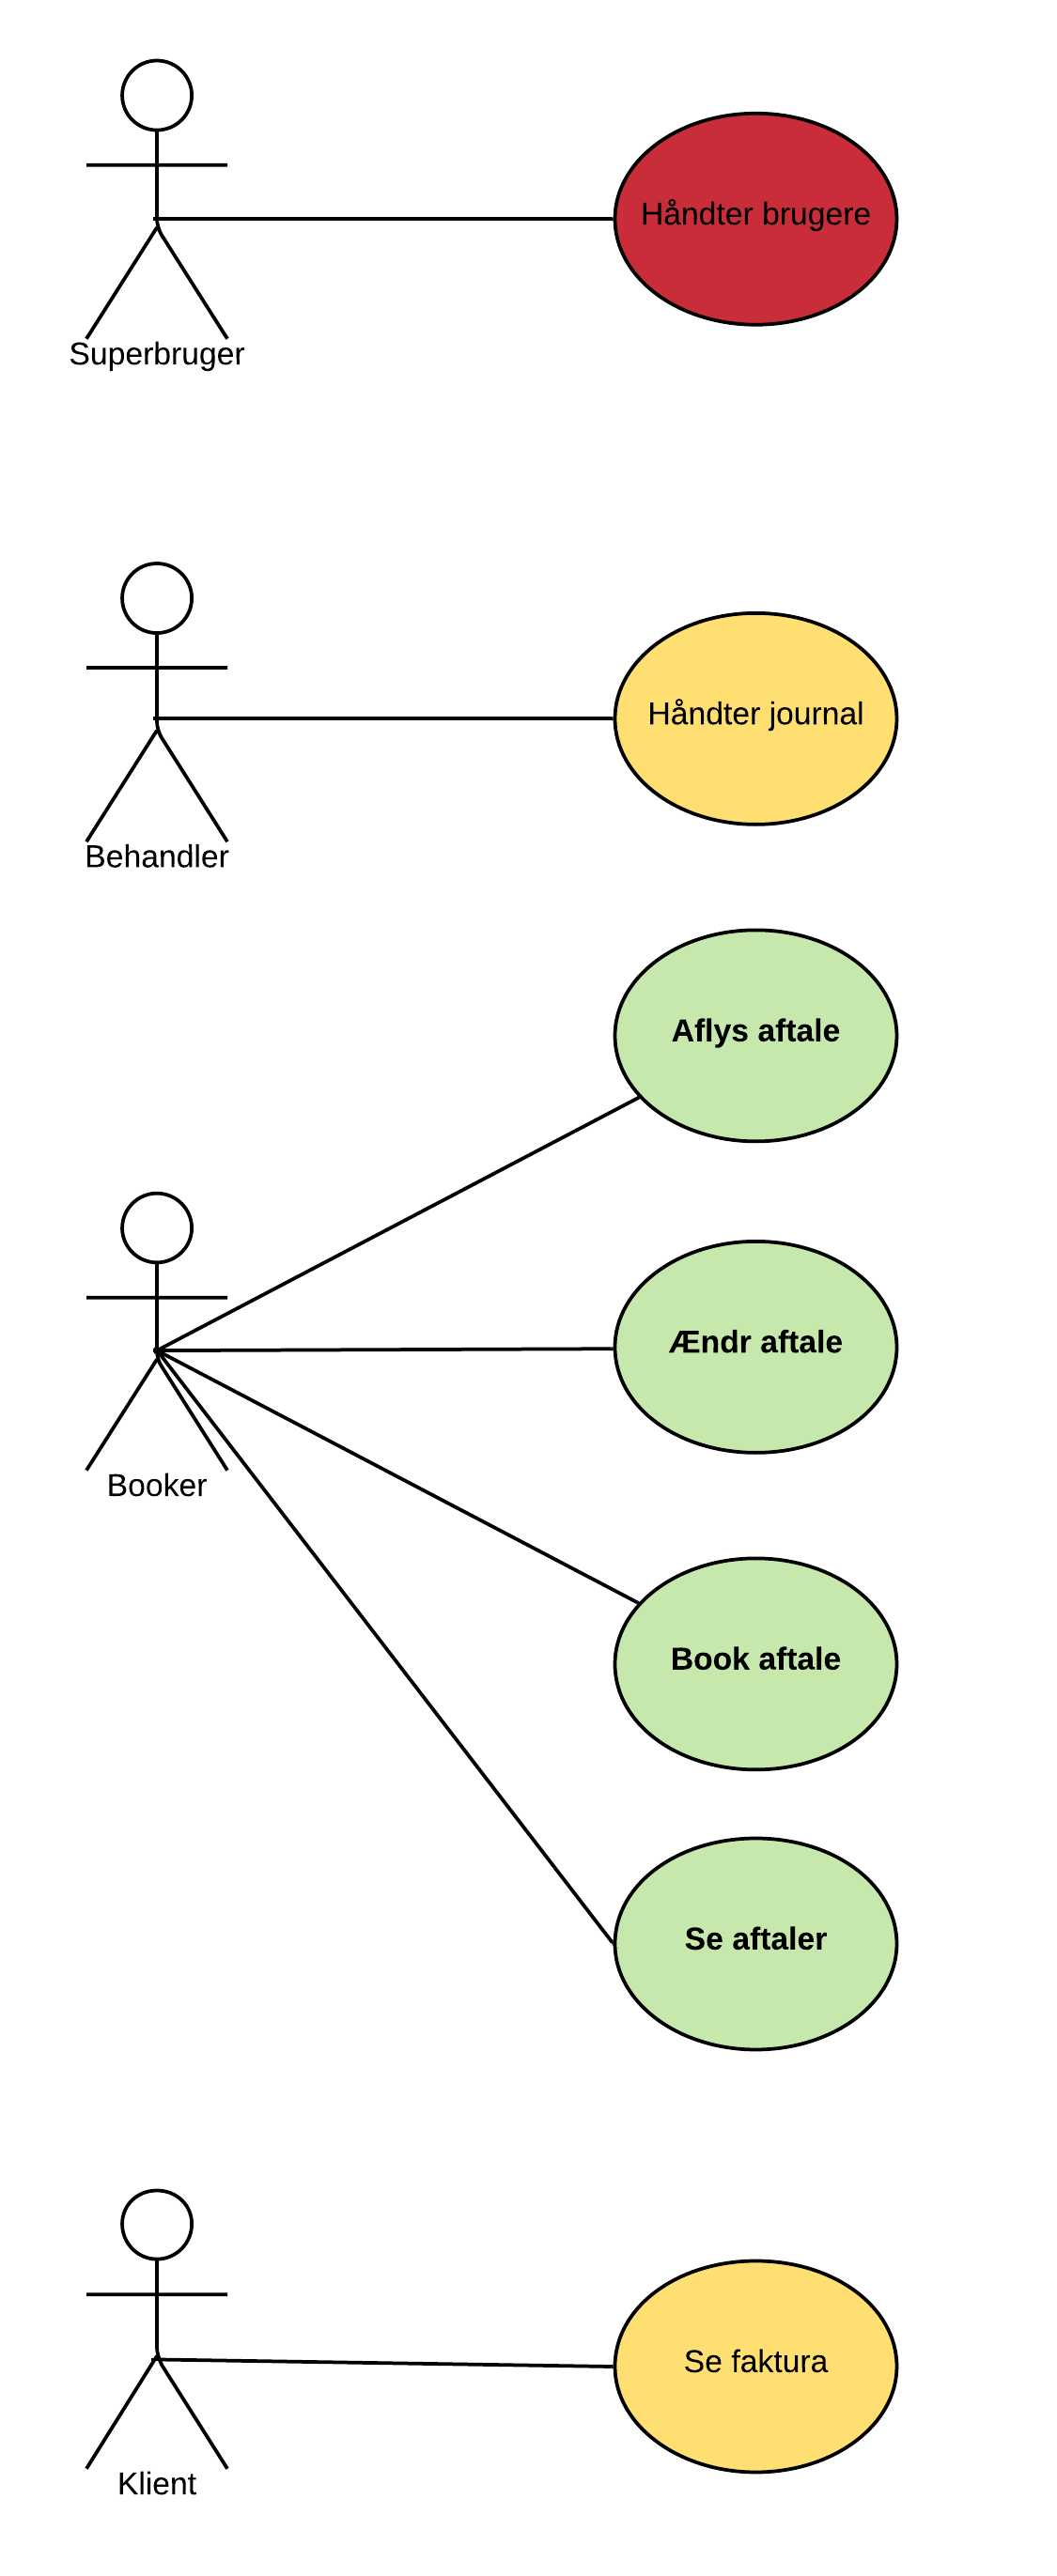
\includegraphics[scale=0.75]{UseCaseDiagram.png}
  \caption{Use Case diagram.}
  \label{fig:UseCaseDiagram}
\end{figure}

På figur \ref{fig:UseCaseDiagram} kan man se alle de use cases vi fandt frem til.
Uses casesne er blevet markeret med farver, der repræsenterer deres prioritering under projektforløbet: de grønne var dem, som Psykolog Nord først ønskede implementeret, derefter gul og tilsidst grøn.
I følgende kapitel kan man så findes vores use cases beskrevet mere detaljeret. 

To personer deltager i en aftale: en klient og en psykolog. Begge udfylder rollen som booker i use casesne med booker som primær aktor, da begge skal kunne håndtere aftaler. 
Vi skelner ikke mellem hvilken af de to aktører, der er bookeren i de nedenstående use cases, da de skal gælde for begge aktører, med mindre der eksplicit står klient eller psykolog.

\subsubsection{Use Case: Book aftale}\label{usecase:bookaftale}
{\setlength{\parindent}{0cm}
\textbf{Scope:} Bookingsystem for Psykolog Nord

\textbf{Primær Aktør:} Booker

\textbf{Preconditions:} En aftale skal ikke eksistere på det givne tidspunkt for begge aftaleparter.

\textbf{Hovedscenarie (succes):} Booking af ny aftale.

Bookeren ønsker at booke en aftale. 
Han vælger at oprette en ny aftale, hvor den anden booker har tid. 
Aftalen oprettes og den anden part notificeres.
}

\subsubsection{Use Case: Ændr Aftale}
{\setlength{\parindent}{0cm}
\textbf{Scope:} Bookingsystem for Psykolog Nord

\textbf{Primær Aktør:} Booker 

\textbf{Preconditions:} En aftale eksisterer, og der er mere end 24 timer til aftalen.

\textbf{Hovedscenarie (succes):} Ændring af aftale.

Bookeren går ind i systemet og ændrer aftalen til andet tidspunkt.
Den anden booker modtager en notifikation med ændringen.
}

\subsubsection{Use case: Aflys Aftale}
{\setlength{\parindent}{0cm}
\textbf{Scope:} Bookingsystem for Psykolog Nord

\textbf{Primær Aktør:} Klient

\textbf{Preconditions:} En aftale eksisterer.

\textbf{Hovedscenarie (success):} Aflysning af aftale.

Den ene booker aflyser aftalen.
Den anden booker modtager en besked om aflysningen og fakturaen, der er tilkoblet aftalen, slettes.

\textbf{Alternativt scenarie:} Aflysning af aftale inden for 24 timer af aftalens tid.

Klienten går ind i system og aflyser aftalen.
Psykologen modtager notifikation om aflysningen, men fakturaen sendes stadig til klienten.

}

\subsubsection{Use Case: Se og betal faktura}
{\setlength{\parindent}{0cm}
\textbf{Scope:} Bookingsystem for Psykolog Nord

\textbf{Primær Aktør:} Klient

\textbf{Precondition:} Faktura eksisterer

\textbf{Hovedscenarie (success):} Se faktura

Klienten går ind i systemet og finder listen over fakturaer. 
Han finder den ønskede faktura og får den vist. Klienten betale derefter fakturaen og modtager kvittering.
}
